\documentclass[12pt, a4paper]{report}

% Packages
\usepackage[utf8]{inputenc}
\usepackage[italian]{babel}
\usepackage{csquotes}
\usepackage[backend=bibtex, style=numeric, sorting=none]{biblatex}	% Bibliografia
\usepackage{listings}	% codice
\usepackage[dvipsnames]{xcolor}	% codice
%gyperref setup
\usepackage{hyperref}
\usepackage{graphicx}
\graphicspath{ {./Immagini} }
\usepackage{wrapfig}
\usepackage{booktabs}

\hypersetup{
    colorlinks,
    citecolor=black,
    filecolor=black,
    linkcolor=black,
    urlcolor=blue	
}


% Titolo
\title{Material Design 3}

\author{
	Ferin Eli \and
	Nardi Marco \and
	Trincanato Marco
}
\date{\today}

% File dove sono scritti tutti i riferimenti bibiografici
\bibliography{resources}

% Syntax highlighting per Kotlin
\lstdefinelanguage{Kotlin}{
  comment=[l]{//},
  commentstyle={\color{gray}\ttfamily},
  emph={filter, first, firstOrNull, forEach, lazy, map, mapNotNull, println},
  emphstyle={\color{OrangeRed}},
  identifierstyle=\color{black},
  keywords={!in, !is, abstract, actual, annotation, as, as?, break, by, catch, class, companion, const, constructor, continue, crossinline, data, delegate, do, dynamic, else, enum, expect, external, false, field, file, final, finally, for, fun, get, if, import, in, infix, init, inline, inner, interface, internal, is, lateinit, noinline, null, object, open, operator, out, override, package, param, private, property, protected, public, receiveris, reified, return, return@, sealed, set, setparam, super, suspend, tailrec, this, throw, true, try, typealias, typeof, val, var, vararg, when, where, while},
  keywordstyle={\color{NavyBlue}\bfseries},
  morecomment=[s]{/*}{*/},
  morestring=[b]",
  morestring=[s]{"""*}{*"""},
  ndkeywords={@Deprecated, @JvmField, @JvmName, @JvmOverloads, @JvmStatic, @JvmSynthetic, Array, Byte, Double, Float, Int, Integer, Iterable, Long, Runnable, Short, String, Any, Unit, Nothing},
  ndkeywordstyle={\color{BurntOrange}\bfseries},
  sensitive=true,
  stringstyle={\color{ForestGreen}\ttfamily},
}

% Altre specifiche per i blocchi di codice
\lstset{
basicstyle=\scriptsize\sffamily\color{black},
frame=single,
numbers=left,
numbersep=5pt,
numberstyle=\tiny\color{gray},
showspaces=false,
showstringspaces=false,
tabsize=1
}











%======================================================================================
%================================ Inizio del report ===================================
%======================================================================================
\begin{document}

% Titolo
\maketitle

% Indice generato automaticamente
\tableofcontents{}



% ===================================================================================
\chapter{Esempi e template}

	\section{Citazioni}
	Ho seguito delle guide per riuscire a far andare la bibliografia, e in sostanza bisogna:
	\begin{itemize}
	\item avere installato il package biblatex
	\item quando si compila, eseguire:
		\begin{itemize}
		\item PdfLatex
		\item bibtex
		\item PdfLatex
		\item PdfLatex
		\item ViewPdf
		\end{itemize}
	\end{itemize}

	Per fare una citazione bisogna:
	\begin{itemize}
	\item aggiungere la risorsa nel file \texttt{resources.bib}
	\item usare il comando \texttt{cite\textbraceleft id\_citazione\textbraceright}
	\end{itemize}

	Le citazioni vengono mostrate automaticamente alla fine del documento con il comando \texttt{printbibliography}

	Qui faremo una citazione di esempio: citazione \cite{example}, \cite{example}

	\section{Blocco di codice}
	Creo un blocco di codice con il syntax highlighting \cite{kotlin_highlight}:
	\begin{lstlisting}[language=Kotlin]
	// this is a simple code listing:
	println("hello kotlin from latex")
	\end{lstlisting}

	Se invece voglio semplicemente una parola in monospace: \texttt{monospace}

	\section{Immagini}
	Per inserire immagini usare il template qui definito

		\begin{figure}[h]
   			\centering
   			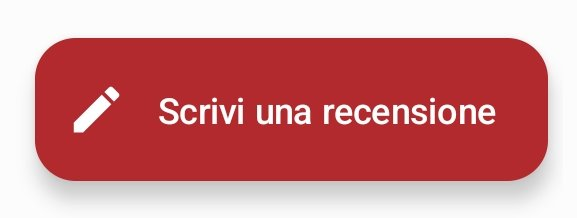
\includegraphics[width=0.3\textwidth]{elevation} %nome del file
 			\caption{Floating Action Button}
    			\label{fig:mesh1} % Se occorre fare un riferimento
		\end{figure}

	Nel Material Design, gli elementi dell'interfaccia utente sono costituiti da \textit{superfici}, ossia delle forme geometriche piatte e dai contorni ben definiti.

		\begin{wrapfigure}{r}{0.3\textwidth}
   			\centering
   			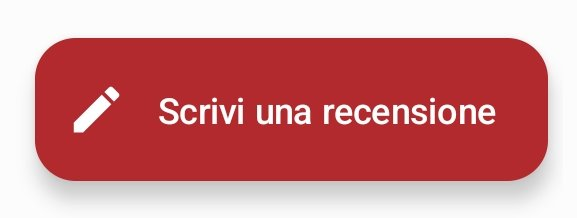
\includegraphics[width=0.3\textwidth]{elevation} %nome del file
		\end{wrapfigure}

		Una superficie può mostrare un contenuto (testo, immagini, icone, ...), che deve essere anch'esso piatto come la superficie su cui si appoggia. Il contenuto può essere indipendente dalla superficie e può cambiare, ma deve sempre rimanere entro i limiti geometrici imposti dalla superficie.

		\begin{wrapfigure}{l}{0.3\textwidth}
   			\centering
   			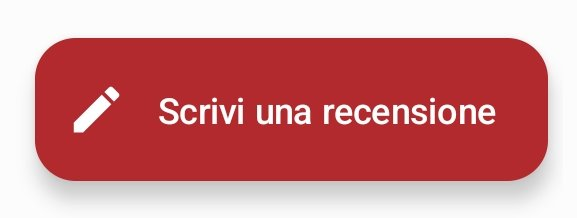
\includegraphics[width=0.3\textwidth]{elevation} %nome del file
		\end{wrapfigure}


		Le superfici si comportano come dei solidi, che possono cambiare forma e opacità, possono unirsi e dividersi, spostarsi e ruotare. Tutti gli elementi della UI del Material Design sono il risutato delle modifiche degli attributi di una superficie di base, che è bianca opaca, di spessore \texttt{1dp}, con un'ombra.





% ======================================================================================
\chapter{Principi del Material Design}

% --------------------------------------------------------------------------------------
	\section{Ambiente}
	L'ambiente del Material Design  \cite{environment} specifica come sono costruiti e come si comportano gli elementi dell'interfaccia utente.

		\subsection{Superfici}
		Nel Material Design, gli elementi dell'interfaccia utente sono costituiti da \textit{superfici}, ossia delle forme geometriche piatte e dai contorni ben definiti.

		Una superficie può mostrare un contenuto (testo, immagini, icone, ...), che deve essere anch'esso piatto come la superficie su cui si appoggia. Il contenuto può essere indipendente dalla superficie e può cambiare, ma deve sempre rimanere entro i limiti geometrici imposti dalla superficie.

		
		Le superfici si comportano come dei solidi, che possono cambiare forma e opacità, possono unirsi e dividersi, spostarsi e ruotare. Tutti gli elementi della UI del Material Design sono il risutato delle modifiche degli attributi di una superficie di base, che è bianca opaca, di spessore \texttt{1dp}, con un'ombra.
		

		\subsection{Elevazione}
		L'elevazione rappresenta la distanza relativa delle superfici lungo l'asse z.

		Lo sfondo ha elevazione 0. Tutte le superfici hanno una elevazione definita in \texttt{dp}. L'elevazione viene visualizzata mediante delle ombre, tanto più intense quanto più grande è il distacco tra la superficie in primo piano e la superficie in secondo piano. Altri modi per mostrare l'elevazione sono l'utilizzo di colori e opacità diversi.

		\begin{figure}[h]
   			\centering
   			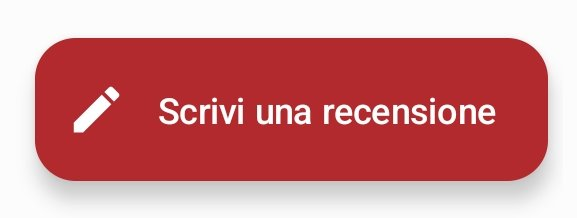
\includegraphics[width=0.3\textwidth]{elevation}
 			\caption{Elevazione in un Floating Action Button}
    			\label{fig:mesh1}
		\end{figure}

		Quando l'utente interagisce con una superficie, la superficie aumenta la sua elevazione, per poi tornare al suo posto quando l'interazione termina. Tutti gli elementi standard hanno una elevazione di default.

		Per evidenziare una superficie in maniera marcata (ad esempio per i messaggi di errore), è possibile oscurare tutto ciò che sta al di sotto della superficie
	
		Le superfici del Material Design non possono occupare la stessa posizione contemporaneamente. Se più elementi devono risiedere nella stessa porzione dello schermo, allora devono avere altezza differente, generando una gerarchia di visualizzazione. Nelle animazioni, le superfici che cambiano elevazione non possono attraversare altre superfici.

		\subsection{Luci e Ombre}
		Nel Material Design delle fonti di luce virtuali illuminano la scena.
		
		Le ombre vengono generate dalla luce che colpisce gli elementi dell'interfaccia utente. L'ombra è tanto più estesa quanto la superficie che colpisce è elevata. Per questo motivo le ombre sono il mezzo con cui si rappresenta la differenza di elevazione tra superfici.


% --------------------------------------------------------------------------------------
	\section{Layout}
		
		\subsection{Anatomia del layout}
		Il Material Design fornisce delle linee guida per ottenere layout che siano intuitivi, consistenti, e reattivi. Ciò è ottenuto attraverso l'uso di griglie, metodi di spaziamento degli elementi, vincoli e altro.\cite{layout_start}

		Il layout è diviso in 3 zone:
		\begin{itemize}
			\item \textit{Body}: mostra la maggior parte del contenuto
			\item \textit{Barra del titolo}: viene usata per mostrare e raggruppare azioni e componenti che
		possono servire all’utente, in relazione al contenuto del \textit{body}
			\item \textit{Barra di navigazione}: permette all'utente di spostarsi tra le varie schermate dell'app
		\end{itemize}

		\subsection{Organizzazione dei contenuti}
			\subsubsection{Raggruppamento visivo}
			Il raggruppamento è uno dei passi fondamentali per creare ordine in un layout: elementi con contenuti o funzionalità simili devono essere raggruppati assieme e separati da altri elementi diversi utilizzando spazi, tipografia o divisori

			\subsubsection{Contenimento}
			Oltre al raggruppamento visivo un altro metodo è contenere assieme elementi che condividono determinate features			\cite{layout_organizzazione}:
			per esempio una notizia avrà un'immagine, un titolo e magari un piccolo paragrafo introduttivo.

			Il contenimento si può ottenere:
			\begin{itemize}
				\item \textit{implicitamente}: lo spazio tra elementi correlati viene ridotto
    			\item \textit{esplicitamente}: gli elementi vengono racchiusi graficamente, ad esempio con una cornice
			\end{itemize}

		\begin{figure}[h]
   			\centering
   			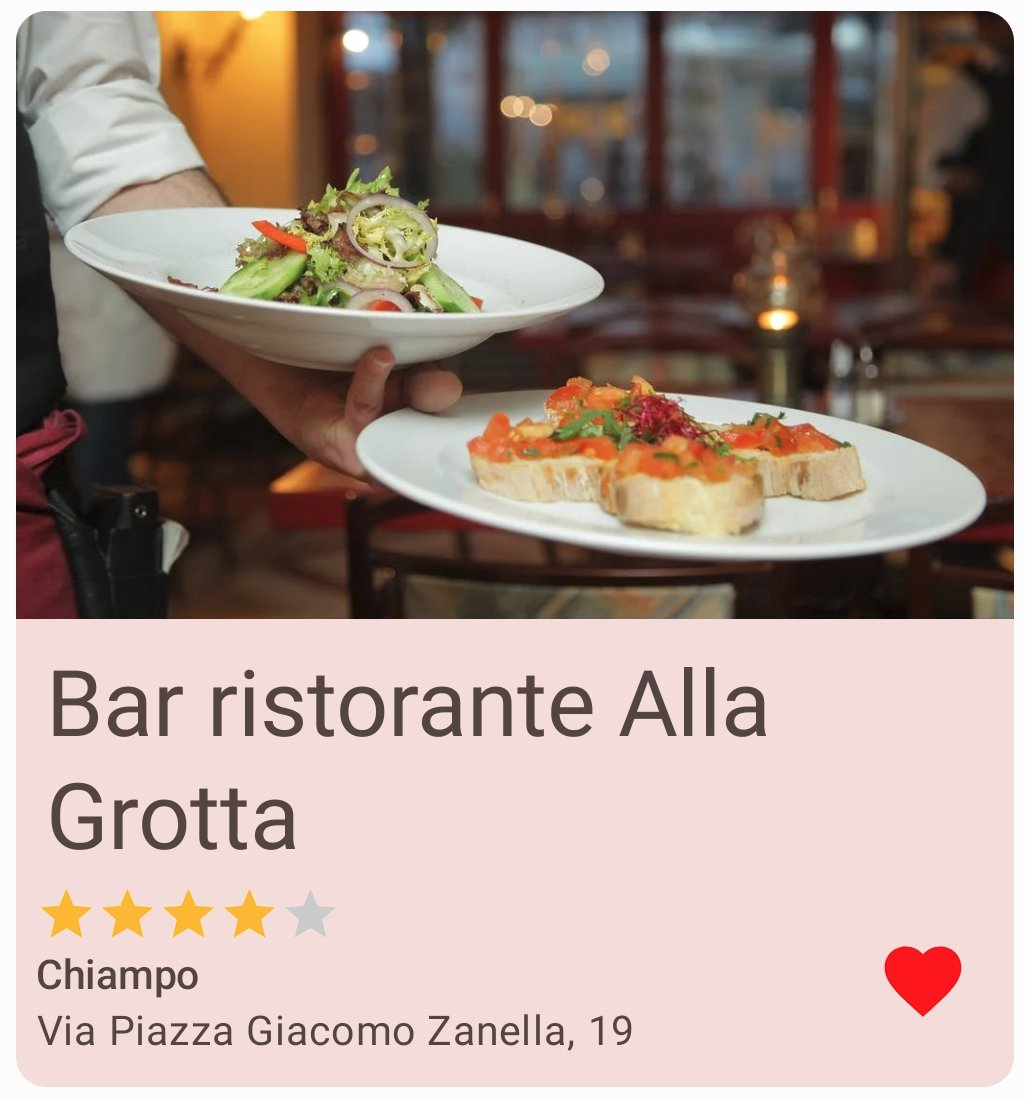
\includegraphics[width=0.4\textwidth]{contenimento}
 			\caption{Le informazioni del ristorante sono racchiuse in una \textit{Card}}
    			\label{fig:mesh1}
		\end{figure}

		\subsection{Misure}
		Le dimensioni degli elementi della UI possono essere misurate in molti modi.

		L'unità di misura più utilizzata è il \textit{density-independent pixel} (\textit{dp}), che permette di mantenere le stesse dimensioni in schermi anche molto diversi tra loro.

		Nel material design in genere si usano multipli di 8 dp per la maggior parte degli elementi della UI. Per elementi molto piccoli si può usare anche 4 dp come unità di base.

		\subsection{Responsive layout grid}
			Il responsive layout grid è un layout in grado di adattarsi a diverse grandezze schermo e orientamenti per garantire consistenza e armonia \cite{layout_grid}

			È composto da:
			\begin{itemize}
				\item \textit{Colonne}: in un dispositivo mobile ce ne sono 4
				\item \textit{Grondaie}: definisco lo spazio che sepra le colonne
				\item \textit{Margini}: definiscono la distanza dal bordo dello schermo
			\end{itemize}

		\subsection{Metodi di spaziatura}
			Per manipolare lo spazio in modo più granulare il layout possono essere utilizzati altri elementi grafici quali:
			\begin{itemize}
				\item \textit{padding}: spazio vuoto che descrive la distanza tra elementi
				\item \textit{allineamenti}: come gli elementi sono allineati nelle righe/colonne
			\end{itemize}

		\subsection{Contenitori e Aspect Ratios}
			Un container rappresenta un'area che contiene elementi di interfaccia utente.
			Possono essere rigidi, che quindi tagliano il contenuto al loro interno nel caso vada oltre i limiti, oppure flessibili, che cambiano la propria dimensione in base al contenuto.

			Per mantenere consistenza nel proprio layout è consigliato l'utilizzo di Aspect Ratios consistenti per elementi come immagini o superfici. Quelli consigliati sono: 16:9; 3:2; 4:3; 1:1; 3:4; 2:3 \cite{layout_containers}

		\subsection{Densità}
			Ci sono casi dove aumentare la densità di informazioni mostrate a schermo può essere utile e rende migliore l'esperienza dell'utente.
			Se l'utente deve interaggire con molte informazioni, si possono rendere le informazioni più compatte diminuendo lo spazio tra loro, rendendole più facili da consultare e confrontare.

			È invece sconsigliato usare una alta densità di contenuti nei componenti che si concentrano nello svolgere un a singola azione (\textit{focused task}) o nei messaggi d'errore

		
% --------------------------------------------------------------------------------------	
	\section{Navigazione}
    	La maggior parte delle applicazioni è composta da più schermate che mostrano all’utente diversi contenuti. È quindi fondamentale che l’utente possa muoversi agevolmente tra queste schermate in maniera rapida e intuitiva.

    	Solitaente esiste una gerarchia tra le schermate di un'applicazione. Questa gerarchia si riflette nell'interfaccia che permette all'utente di navigare.

    		\subsection{Navigazione laterale}
    		La navigazione laterale viene utilizzata per spostarsi tra pagine allo stesso livello nella gerarchia.

    		Solitamente viene implementata con una \textit{bottom navigation bar} (preferita nei dispositivi mobili) o con un \textit{navigation drawer}.

    		Per schermate di gerarchia più bassa possono essere utilizzate le \textit{tabs}.

    		\begin{figure}[h]
   			\centering
   			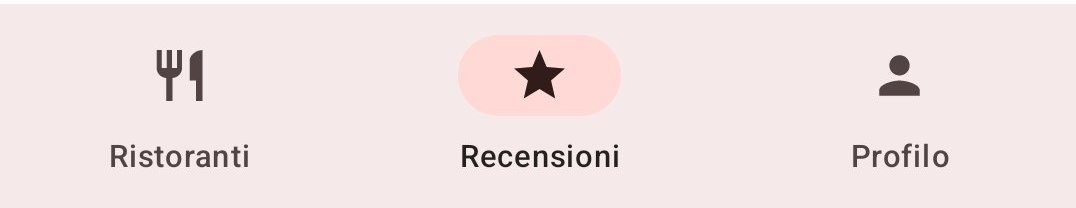
\includegraphics[width=0.5\textwidth]{navbar}
 			\caption{Barra di navigazione}
    			\label{fig:mesh1}
		\end{figure}

    		\subsection{Navigazione in avanti}
    		La navigazione in avanti viene utilizzata quando l'utente si sposta tra schermate a livelli consecutivi di gerarchia. Si utilizza la navigazione in avanti ogni volta che si utilizzano pulsanti, collegamenti, ricerche.

    		A differenza della navigazione laterale, quella in avanti non prevede elementi dell'interfaccia utente dedicati.

    		Associata alla navigazione in avanti è la navigazione all'indietro, che permette all'utente di ritornare alla schermata cronologicamente precedente oppure ad un livello gerarchico superiore.


    		\subsection{Navigation transitions - da tenere se implementiamo nell'app}
    		Le transizioni di navigazione si verificano quando gli utenti si spostano tra le schermate e utilizzano il movimento per guidare gli utenti tra due schermate nell'app. Aiutano gli utenti
    		a orientarsi esprimendo la gerarchia dell'app, usando il movimento per indicare in che modo gli elementi sono correlati tra loro. Il material design definisce 2 macro tipi di transizioni:
    		\begin{itemize}
    			\item \textit{Hierarchical transitions}. Si usano quando gli utenti salgono o scendono di un livello in un'app. Gli schermi a livelli adiacenti tra loro hanno una relazione genitore e
    			figlio l'uno con l'altro, in cui il genitore si trova a un livello gerarchico più alto rispetto al figlio. Nelle transizioni padre-figlio, un elemento figlio presente nello schermo padre
    			si solleva al tocco e si espande sul posto, utilizzando un modello di transizione di trasformazione del contenitore. Il movimento attira l'attenzione sullo schermo figlio (che è la destinazione
    			dell'interazione), mentre rafforza la relazione tra gli schermi genitore e figlio.
    			\item \textit{Peer transitions}. Si verificano tra le schermate allo stesso livello di gerarchia. Le transizioni tra pari si verificano tra schermate che condividono un genitore, mentre le transizioni tra pari
    			di livello superiore vengono utilizzate solo per passare da una destinazione primaria all'altra. Si distinguono 2 tipi di peer transition:
    			\begin{itemize}
    				\item \textit{Sibling transitions}. Gli schermi che condividono lo stesso genitore (come le foto in un album, sezioni di un profilo o passaggi in un flusso) si muovono all'unisono per
    				rafforzare la loro relazione reciproca. Lo schermo del peer scorre da un lato, mentre il suo fratello si sposta fuori dallo schermo nella direzione opposta.
    				\item \textit{Top-level transitions}. Al livello superiore di un'app, le destinazioni sono spesso raggruppate in attività principali (e le attività potrebbero non essere correlate tra loro).
    				Queste schermate si aprono utilizzando uno schema di transizione di dissolvenza.
    			\end{itemize}
    		\end{itemize}
	
	
% --------------------------------------------------------------------------------------
	\section{Colori}
	Il Material Design definisce delle \textit{palette} di colori, con lo scopo di armonizzare e rendere piacevole alla vista ciascun elemento delle app.
	
	Per ciascuna palette sono definiti dei colori specifici per ciascun ruolo degli elementi della UI:
	\begin{itemize}
		\item \textit{primary}: indica il colore principale degli elementi dell'app, viene utilizzato per gli elementi della UI come la barra di navigazione
		\item \textit{secondary}: indica un colore alternativo, per distinguere gli elementi della UI vicini tra loro (uno di colore primario e uno di colore secondario)
		\item \textit{primaryVariant} e \textit{secondaryVariant}: sono delle versioni leggermente alterate da utilizzare quando più elementi si sovrappongono o hanno importanza diversa
		\item \textit{background}: colore dello sfondo
		\item \textit{surface}: colore di default delle superfici di menu, cards, ...
		\item \textit{error}: colore per i messaggi d'errore
		\item Colori \textit{on[...]}: da applicare al testo e alle icone che si trovano su un determinato colore di sfondo. Questi colori garantiscono un adeguato contrasto con lo sfondo stesso
		\begin{itemize}
			\item \textit{onPrimary}
			\item \textit{onSecondary}
			\item \textit{onBackground}
			\item \textit{onSurface}
			\item \textit{onError}
		\end{itemize}
	\end{itemize}
	
		\subsection{Temi}
		Dato un colore \textit{primary}, può essere definita una palette di colori coerente con il colore scelto.
		
		In particolare il Material Design indica delle linee guida per generare una palette per il \textit{tema chiaro} e una per il \textit{tema scuro}. Quest'ultima è generata desaturando i colori per il tema chiaro, così da renderli più leggibili su superfici scure.

		I colori particolarmente adatti alle linee guida del Material Design sono forniti dal \href{https://material.io/resources/color/#!/?view.left=0&view.right=0&primary.color=6002ee}{Color Tool} \cite{color_tool}

% --------------------------------------------------------------------------------------   
   \section{Suono}
   	    Il suono viene usato per migliorare l'esperienza dell'utente: comunica un feedback utile, assegnando personalità e
   	    perfezionando l’estetica del prodotto.

   	    In un'interfaccia utente, si distinguono tre tipologie di suono: \textbf{sound design}, \textbf{musica} e \textbf{voce}. Ogni tipologia comunica informazioni e \textit{brand identity} in modi diversi.

   	    Il \textbf{sound design} viene utilizzato principalmente per associare un elemento dell'interfaccia utente a un suono specifico e far capire qual è la struttura gerarchica.
		Tuttavia, si usa anche per esprimere personalità o fornire feedback.


        La \textbf{musica} viene utilizzata principalmente per la narrazione ed esprime uno "stato d'animo" dell'interfaccia utente.
        Se abbinata a immagini o transizioni, la musica può elevare la narrativa e le sensazioni generali di un prodotto.



        La \textbf{voce} e la sintesi vocale utilizzano entrambe il linguaggio parlato per comunicare informazioni dove il sound
        design e la musica non sono abbastanza.

        \subsubsection{Quando non usare il suono}
                	Il silenzio nel design dell'interfaccia utente è importante tanto quanto il suono. In molti casi, l’audio non è necessario e può,
                    ridurre il comfort dell'utente. Il suono, di solito, non è adatto per UI che richiedono privacy e per azioni eseguite di frequente.


              \subsubsection{Tipi di suono}
				\begin{itemize}
					\item \textbf{Hero sound}: si verificano in interazioni fondamentali, evocando uno stato emotivo o celebrando un certo tipo di eventi;
					\item \textbf{Notifiche}: aiutano a dirigere l'attenzione dell'utente, più brevi degli hero sound e realizzate affinché possano essere riprodotte più volte;
					\item \textbf{Suoni di sistema}: divisi in:
					\begin{itemize}
						\item \textit{suoni UX primari}: generati da un sistema operativo (o dispositivo) per fornire feedback agli utenti;
						\item \textit{suoni UX secondari}: riprodotti meno frequentemente e utilizzati principalmente per scopi	funzionali.
					\end{itemize}
					\item \textbf{Suoni ambientali}: creano atmosfera senza distogliere l'utente dall'attività, in genere basati su musica o suoni ambientali
				\end{itemize}

				\subsection{Formato dei file e ottimizzazione della memoria}
				La riproduzione del file audio può variare a causa delle limitazioni hardware e software di un dispositivo. Per ridurre le dimensioni del file si usano diversi metodi,
				come la compressione con perdita o la riduzione della frequenza di campionamento.

				Il formato finale dell'audio dipende dall'implementazione e dalle restrizioni a livello di sistema. Quindi, di solito si sceglie il formato più lossless consentito dal sistema.



% --------------------------------------------------------------------------------------
	\section{Tipografia}
		Il material design fornisce molti strumenti per poter scegliere il font adatto con le misure giuste per ogni tipo di testo, forniscono pure un \href{https://material.io/design/typography/the-type-system.html#type-scale}{Type scale generator} che permette di creare il proprio type scale.
		Vengono fornite misure e conversioni per Android, iOS e Web; e misure per titoli, sottotitoli e corpi di testo.

		\subsection{Dimensioni}
		Le categorie di testo individuate dal Material Design sono
		\begin{itemize}
			\item \textit{headline}: con 6 dimensioni disponibili, headline vien utilizzata per i titoli
			\item \textit{sottotitoli}: più piccoli dei titoli, sono sempre di breve lunghezza
			\item \textit{corpo}: viene utilizzato per il contenuto testuale dell'app, che può essere anche molto lungo
			\item \textit{testo per i pulsanti}: in genere con sole lettere maiuscole, è dedicato ai pulsanti
			\item \textit{didascalie e overline}: sono i type scale più piccoli. Didascalie spesso servono per annotare degli elementi mentre overlines a introdurre dei titoli.
		\end{itemize}

	\subsection{Proprietà di un typeface}
		Le proprietà che caratterizzano un typeface o permettono di modificarne le misure sono
		\begin{itemize}
			\item \textit{baseline}: è una linea invisibile che definisce come i songoli caratteri si allineano sulla griglia (ad esempio definisce quanto sono grandi le lettere maiuscole rispetto alle minuscole)
			\item \textit{peso}: rappresenta lo spessore del tratto dei caratteri. Assume valori da 1 (\textit{light}) a 4 (\textit{bold})
		\end{itemize}

	\subsection{Leggibilità}
	La leggibilità di un testo è determinata da molteplici fattori quali
	\begin{itemize}
		\item \textit{letter spcing}: si riferisce allo spazio tra le lettere che compongono una parola, a seconda della funzione del testo si posson usare spazi più piccoli o grandi
		\item \textit{tabulazione}: aiuta a leggere cifre lunghe quando sono vicine ad altre, come per esempio in colonna in una tabella
		\item \textit{lunghezza e altezza delle righe}
	\end{itemize}




% --------------------------------------------------------------------------------------
	\section{Iconografia}
		Il material design fornisce strumenti, griglie e specifiche per utilizzare e creare le proprie icone, con l'obbiettivo di mantenere un certo livello di semplicità.
		\subsection{Design delle icone}
			Nel Material Design, le icone sono realizzate per essere semplici e moderne, ridotte alla forma minima, esprimendo solo concetti essenziali, con forme geometriche semplici e consistenti. Questa semplicità permette alle icone di rimanere leggibili e distinguibili anche a dimensioni piccole.

			\subsubsection{Dimensioni}
			Le icone sono normalmente 24dp x 24dp, nel caso di layout più densi come su un desktop possono essere scalate a 20dp x 20dp.
			Per ogni icona vi è un perimetro di padding di 2dp,per prevenire sovrapposizioni o oscuramenti in layout densi o nel caso appaiano altri elementi a schermo.

			Vengono fornite delle keylines e griglie per il design di icone: principalmente vengono usati quadrati, cerchi e rettangoli.
			Il tratto che si usa quando si crea la propria icona deve essere sempre spesso 2dp, questo mantiene consistenti le icone, i tratti finali di un'icona, per esempio la punta di una freccia, sono sempre dritti e non tondi.

			\subsubsection{Orientamento}
			Le icone devono sempre guardare avanti, non vanno girate o piegate, e devono sempre apparire piatte e non tridimensionali.
			L'opacità di un'icona dipende dallo sfondo e dal suo stato: attiva o inattiva.

			\subsubsection{Transizioni}
				Le transizioni sono effetti tra due icone, quando si preme un'icona viene eseguita l'animazione e l'altra icona diventa visibile o attiva, per esempio cliccando l'icona \textit{pausa} in un lettore di musica, la musica si ferma e l'icona diventa \textit{riprendi}.
				Le animazioni possono essere semplici (una semplice rotazione), o complesse (trasformazioni e altri effetti), spesso se la funzionalità è più importante dell'aspetto visivo si scelgono animazioni semplici.
				La durata di un'animazione semplice (come un pulsante on/off) è di 100ms, animazioni un po' più complesse 200ms (per esempio una rotazione), per animazioni che fanno uso di molte trasformazioni si usano 500ms così da poter vedere bene l'animazione.

% --------------------------------------------------------------------------------------
	\section{Forme}
	Gli elementi di un’applicazione possono essere visualizzati attraverso diverse forme. Le forme dirigono l'attenzione, identificano i componenti, mostrano come le superfici si relazionano tra loro ed esprimono il brand.


	Le componenti hanno una forma rettangolare per impostazione predefinita, con angoli arrotondati di 4 dp (density pixel). La loro forma può essere personalizzata regolando dimensione e forma degli angoli.

	La forma di alcuni componenti di un’applicazione viene modificata per vari motivi: le forme con un design unico (\textit{forme uniche}) differiscono dalle forme che le circondano e dall'interfaccia utente nel suo insieme, aiutando a dirigere l'attenzione dell'utente.
	Inoltre, una forma diversa rispetto alle altre componenti di quel gruppo può comunicare il cambiamento di stato di una componente utilizzando .

	Ancora, per esprimere il linguaggio visivo di un \textbf{marchio} in un'app, si usano le forme insieme ad altre personalizzazioni, come colore e tipografia, in modo coerente.
	Queste piccole modifiche alla forma, applicate strategicamente, contribuiscono all'impressione generale che un brand da all’utente.


	\subsection{Gruppi di forme}
	I componenti sono raggruppati in gruppi di forme in base alle loro dimensioni. In questo modo, si possono modificare contemporaneamente più valori di un gruppo di componenti. I gruppi di forme includono:
	\begin{itemize}
		\item \textit{Componenti piccoli}, come pulsanti, chip, campi di testo, snackbar;
		\item \textit{Componenti medi}, come menu, card, dialog;
		\item \textit{Componenti grandi}, come sfondi, tabelle, drawer
	\end{itemize}


	I gruppi di forme utilizzano degli attributi per definire la forma da assegnare agli angoli dei componenti. È possibile personalizzare i seguenti attributi:
	\begin{itemize}
		\item \textit{tipo di angolo}: appuntito, arrotondato, tagliato;
		\item \textit{dimensioni}: il raggio dell'angolo. Può essere assoluto (in dp) oppure in funzione delle dimensioni della forma stessa;
		\item \textit{simmetria}: è possibile applicare modifiche solo ad angoli specifici.
	\end{itemize}

	Per applicare una famiglia di forme e una dimensione a tutti i componenti di un gruppo, bisogna impostare i valori per il gruppo di forme. Quando vengono apportate modifiche a un gruppo, le modifiche influiscono su tutti i componenti in quel gruppo di forme, ad eccezione di quelli con una sostituzione.

	\subsection{Uso efficace delle forme}
	Le forme sono visibili quando i bordi della superficie hanno un contrasto sufficiente rispetto allo sfondo. Per impostazione predefinita, il Material Design rende visibili le forme utilizzando le ombre per visualizzare i bordi delle superfici.
	Tuttavia, esistono altri metodi per rendere visibili le forme, come riempimenti di colore e opacità, che possono essere utilizzati in combinazione con le ombre o da soli.

	Le forme aiutano gli utenti a identificare i componenti e influiscono sulla loro usabilità.

	La forma può comunicare molte informazioni su un elemento, incluso il suo stato corrente, il risultato di un'interazione dell'utente o altre modifiche in un'app. Se utilizzata in questi modi, la forma dovrebbe essere presentata in modo coerente
	nello stesso stato e nelle stesse interazioni, in modo che una forma specifica abbia lo stesso significato ogni volta che viene incontrata.

	Se una forma non è interattiva, è necessario evitare l'utilizzo di forme con dimensioni sufficientemente grandi da apparire interattive. Ad esempio, una piccola forma triangolare su una card non dovrebbe essere abbastanza grande da essere scambiata per un elemento da toccare, se non lo è.

	\subsubsection{Branding}
	La combinazione di stili e forme diverse può rendere difficile l'associazione di forme particolari a un marchio. Per esprimere l'identità di un brand, si identifica la forma distintiva del marchio, ad esempio una forma organica o geometrica che riflette
	gli attributi del logo. Sulla base di questa forma,  viene poi sviluppata una serie di forme simili da applicare al prodotto che contribuiscono a unificare l'espressione del marchio in tutta l'applicazione. Tuttavia, l'uso eccessivo della forma per esprimere il marchio può portare
	alla diluizione dello stesso: la forma perde la sua connessione con il marchio e diventa un luogo comune. Inoltre, troppe forme uniche possono portare a nessuna forma particolarmente prominente, nonché a una mancanza di coesione visiva tra i componenti.

	\subsubsection{Angoli}
	E' necessario evitare di utilizzare valori percentuali per i componenti che modificano dinamicamente la propria altezza, altrimenti la forma potrebbe modificarsi in modi inaspettati.
	Inoltre, gli angoli ancorati ai bordi dello schermo non possono essere personalizzati, altrimenti si creerebbero spazi vuoti che lasciano trasparire il contenuto dietro ad un componente.

	\subsubsection{Modifiche ad altri sistemi}
	Le personalizzazioni del sistema possono influire sull'uso della forma da parte di un componente. Ad esempio, l'aumento della dimensione del carattere potrebbe causare il taglio di parte di un testo e la modifica di altezza e forma del componente, se le dimensioni sono definite come percentuali.
	Le modifiche al contenuto possono anche influire sulla forma di un componente. Ad esempio, se la lunghezza del testo aumenta, il testo potrebbe andare a capo su una riga aggiuntiva, aumentando l'altezza del componente e influenzando le forme definite come percentuale.

	\subsubsection{Morphing}
	Gli elementi possono cambiare forma in risposta alle modifiche al contenuto o all'interazione dell'utente. Questa trasformazione si chiama \textit{morphing}. Le forme possono trasformarsi per vari motivi: in risposta a cambiamenti di stato o contenuto o come risultato dell'interazione dell'utente. Ad esempio, quando si ruota un
	dispositivo mobile da verticale a orizzontale, le superfici possono rispondere modificando le dimensioni, il che può causare la trasformazione delle forme.

	Il morphing di una forma dovrebbe preservare le proporzioni delle forme distintive, per evitare la distorsione.
	Inoltre, tutto il contenuto su una superficie dovrebbe essere visibile mentre la superficie si trasforma, senza ritagliare il contenuto.

	\subsection{Collegare superfici attraverso le forme}
	Le forme possono aiutare gli utenti a capire in che modo le superfici sono correlate tra loro.
	Forme simili possono indicare che le superfici sono dello stesso tipo, come le carte in una raccolta con dimensioni e angoli corrispondenti.

	Le superfici correlate tra loro possono essere indicate utilizzando forme che ricordano le frecce, in modo tale da "puntare" verso altre superfici. Ad esempio, un angolo a forma di freccia di un menu può puntare a una superficie correlata.


	Le forme possono enfatizzare le superfici separate l'una dall'altra. Ad esempio, quando una forma unica appare a un'altezza maggiore rispetto a un'altra superficie, si sottolinea che le due superfici sono separate.

	\subsection{Forme nel material design 3}
	Il material design tre intoduce un cambiamento ai gruppi di forme, sempre basati sulle dimensioni, ma con con sette stili degli angoli, assegnati in base alla quantità di arrotondamento desiderata. Le forme con angoli squadrati sono chiamate "none", le forme leggermente arrotondate sono "extra-small", mentre le forme completamente arrotondate sono "full".
	Ciò consente di conferrire maggior espressività all'interfaccia utente. Viene, inoltre, mantenuta la possibilità avere forme degli angoli simmetriche o asimmetriche, con angoli tagliati o arrotondati. Inoltre, è sempre modificare lo stile di un' intera categoria di forme

% --------------------------------------------------------------------------------------
	\section{Interazione}

		\subsection{Gesture}	
		Le \textit{gestures} permettono all'utente di interagire con gli elementi dello schermo in maniera rapida e intuitiva.
		
		Gli elementi con cui è possibile interagire hanno degli accorgimenti grafici che permettono all'utente di intuire la gesture da eseguire e il suo effetto nello schermo
		
			\subsubsection{Gesture di navigazione}
			Le gesture di navigazione permettono all'utente di spostarsi tra le schermate dell'app:
			\begin{itemize}
				\item \textit{tap}: la schermata cambia quando viene toccato un elemento
				\item \textit{scroll and pan}: la schermata scorre seguendo il tocco dell'utente
				\item \textit{drag}: permette all'utente di spostare elementi per visualizzarli o nasconderli
				\item \textit{swipe}: permette la navigazione orizzontale tra schermate
				\item \textit{pinch}: modifica le dimensioni delle superfici della UI
			\end{itemize}
			
			\subsubsection{Gesture di azione}
			Le gesture si azione permettono all'utente di eseguire azionie avere accesso a ulteriori funzionalità
			\begin{itemize}
				\item \textit{tap}: esegue azioni di base, come la navigazione 
				\item \textit{long press}: permette di accedere a azioni e modalità generalmente nascoste e poco accessibili
				\item \textit{swipe}: permette di eseguire velocemenete azioni quando viene superato un certo \textit{threshold}. Viene generalmente utilizzata nelle liste
			\end{itemize}
			
			\subsubsection{Gesture di trasformazione}
			Le gesture di trasformazione permettono di spostare, ridimensionare, ruotare gli elementi della UI
			\begin{itemize}
				\item \textit{double tap}: permette di ingrandire e rimpicciolire il contenuto della schermata. Ha una funzionalità molto simile al \textit{pinch}
				\item \textit{compound gestures}: sono delle gestures che permettono di combinare spostamenti, zoom e rotazioni. Vengono spesso utilizzati nelle mappe
				\item \textit{pick up and move}: combina un \textit{long press} con un \textit{drag}. Ha lo scopo di riordinare gli elemeti di un insieme ordinato
			\end{itemize}

		\subsection{Selezione}
		La selezione permette di specificare gli elementi della schermata su cui si vuole eseguire una determinata azione.

		Nei dispositivi touch, la selezione viene effettuata con un \textit{long press}, oppure con delle \textit{selection mode} da cui è possibile selezionare gli elementi con un \textit{tap}.
		
		Quando un elemento viene selezionato, l'utente riceve un feedback, sotto forma di spunta o di un cambiamento di colore dell'elemento stesso.
		
		\subsection{Stato}
		Lo stato di un componentte viene visualizzato mediante una varizione del suo aspetto.
		
		Le variazioni associate a ciascuno stato devono essere:
		\begin{itemize}
			\item \textit{distinguibili}: ogni stato deve essere riconoscibile
			\item \textit{additive}: se più stati sono presenti nello stesso momento, tutti devono essere rappresentati
			\item \textit{consistenti}: devono essere le stesse indipendentemente dal componente su cui sono applicate
		\end{itemize}
		
		Inoltre, le variazioni devono sempre garantire la leggibilità e l'armonia generale delle componenti
		
			\subsection{Tipi di stato}
			I tipi di stato che generalemnte vengono rappresentati sono:
			\begin{itemize}
				\item \textit{enabled/disabled}: indica se è possibile interagire con il componente
				\item \textit{hover}: indica se il cursore è posizionato sopra il componente. Suggerisce che è possibile un'interazione
				\item \textit{focused}: indica che il componente è evidenziato da un sistema di input diverso dal tocco (ad esempio un assistente vocale o una tastiera esterna)
				\item \textit{selezionato}: indica se l'utente ha selezionato il componente
				\item \textit{attivato}: indica, generalmente in una lista, con quale componente si sta interagendo
				\item \textit{premuto}: tipico dei pulsanti, indica che l'utente ha premuto con un \textit{tap} il componente
				\item \textit{trascinato}: indica se l'utente sta trascinando il componente con un \textit{drag}
				\item \textit{on/off}; tipico di \textit{switch} e \textit{checkbox}, indica lo stato booleano del componente
				\item \textit{error}: indica che qualcosa non va
			\end{itemize}
% --------------------------------------------------------------------------------------		

	\section{Motion}
		Le transizioni aiutano l'utente a capire quali elementi sono correlati, e rendono l'interfaccia utente più bella da vedere.
		Animazioni in loghi, icone, immagini possono dare feedback all'utente per delle azioni, per esempio premere un pulsante fa partire un'animazione che mostra che sia stato effettivamente premuto.
		Le animazioni possono anche insegnare all'utente come fare una certa azione: l'azione swipe to unlock è animata mostrando la schermata che effettivamente scorre verso l'alto.
		\subsection{Transition patterns} 
			Material design fornisce delle patterns per transitions e sono:
			\begin{itemize}
				\item Container transform
				\item Shared axis
    			\item Fade through
				\item Fade
			\end{itemize}
		Per scegliere quale pattern usare vengono fornite delle linee guida:
		\subsubsection{Container transform}
			Nel caso siano presenti dei container che rimangono visibili a schermo durante tutta la transizione (sono appunto chiamati persistent), è consigliato l'utilizzo di una container transform.
			Come mostrato \href{https://kstatic.googleusercontent.com/files/ba0be42ae71266d6e68503fe131ff522c906a23622af8dd6cddc06f55daaf9366e9431df3645d9328b9acf84674f526c59a67d91b5ea49ef63a7404b3b95fe47}{qui}
			il container transfrom è molto utile per mostrare relazioni tra elementi, come per esempio una scheda e i suoi dettagli.
			Ne esistono diverse varianti ma tutte hanno in comune il container che aprendosi si allarga a determinate dimensioni (schermo intero o anche u piccolo menù).
		\subsubsection{Shared axis}
			Gli elementi collegati sia dal punto di vista semantico che spaziale, possono essere animati attraverso una \textit{shared transformation}: gli elementi che escono ed entrano si muovono allo stesso modo attraverso un asse deciso come mostrato \href{https://kstatic.googleusercontent.com/files/d2e9627f4006e27d36d8e839d2f3f92f1de59558bebdbe725ce5b2e0bd8a0a8c32285e10aceb52431be2e61acf003fba809ddd8bbd464ee8256bad0eee98e9a1}{qua}.
			A seconda dell'asse utilizzato si possono avere diversi significati, per esempio procedere avanti attraverso un form da compilare può essere visto come un'animazione orizzontale, che rappresenta lo scorrimento di una pagina.
		\subsubsection{Fade Through}
			Elementi che non sono collegati possono essere animati con un semplice fade through. Questa animazione è spesso usata per elementi come destinazioni di navigation bars.
		\subsubsection{Fade}
			Il fade è utilizzato per elementi che entrano lo schermo utilizzandone solo una parte, come un \href{https://kstatic.googleusercontent.com/files/4bf2ddbf50d779f37d88f276b831fad1aad78a23379a87d2b715dbb90d878897d1ad5edcf03385e1814d2ec3f4e9f152fd736ab2727d7f0e0d8b58467eb41057}{menù delle opzioni}.
	\subsection{Velocità}
		La velocità di una transizione è molto importante perchè se è troppo veloce l'utente non capisce cosa sta accadendo, mentre se è troppo lenta rallenta anche l'esperienza dell'utente.
		Per modificare la velocità si possono cambiare durata e \textit{easing} (accelerazione). Vengono fornite anche qua delle linee guida in base al tipo di transizione:
		\subsubsection{Chiusura}
		Transizioni che chiudono elementi, o tornano indietro devono essere corte in quanto richiedono meno attenzione dall'utente.
		Elementi piccoli o di poca importanza hanno anche loro transizioni che durano poco.
		\subsubsection{Elementi grandi}
		Elementi che occupano grande parte dello schermo sono quelli che devono avere animazioni più lunghe
		\subsubsection{Easing}
		L'easing permette alle transizioni di accelerare o rallentare rendendole più naturali e meno rigide.Come si vede \href{https://kstatic.googleusercontent.com/files/cd28926c3e6b98926788199361bc3e613f6fd98234fa12e143fe528ba629f0ee7318c16acf5a389820d4789f43c12b011880909e39a59d73377a5a1c270bbe52}{qua}
		l'easing rende il movimento del puntino molto più naturale.
		Ne esistono diversi tipi:
		\begin{itemize}
			\item \href{https://kstatic.googleusercontent.com/files/c60193433c491a0ea5b95fd2740fab851ff3572e5191ceab47a9a9586262a6bf354baa78f19b1bdbaca0674562971cec7d0e8e45f56e8d79dadd95329ed907d5}{Standard}
			\item \href{https://kstatic.googleusercontent.com/files/1b3b1c294a5075226c259f5af1569e9e79606bd65ddb27afa1ccf4815d627c6c9b6c787d59a7bb26861694727a30e6fcf5d4def3388d973920339d25aca6c8f3}{Emphasized}
			\item \href{https://kstatic.googleusercontent.com/files/b624b31824d5a199f82de3273246101bf20dbb079c3a81a2b7b66bf6ef96ac97808fc8f27180310345f977aae93c2581a1f9280963c92ed71c95107583fe3d9a}{Decelerated}
			\item \href{https://kstatic.googleusercontent.com/files/4e2afcefc0aa8b74bdd1980114e5e8bd8b7b13e7944c17f9710731c22fed2f80e89edb91ec904a14d511a469de73f487836f86e0c91f0e98f31419ed3106a408}{Accelerated}
		\end{itemize}

% --------------------------------------------------------------------------------------
	\section{Comunicazione}
	\subsection{Confirmation and acknowledgement}
	Le comunicazioni di \textbf{conferma} e \textbf{acknowledgement} chiedono l’autorizzazione all’utente prima di intraprendere un'azione e gli confermano la riuscita delle stesse.

	Le azioni di \textit{conferma}  chiedono all'utente se desidera procedere con l'azione appena eseguita. Possono essere associate a un avviso o ad informazioni critiche relative a tale azione. La conferma non è necessaria quando le conseguenze di un'azione sono reversibili o trascurabili.
	La richiesta viene rese al meglio utilizzando una finestra di avviso (alert dialog).

	Le azioni di \textit{acknowledgement} forniscono un testo per far sapere all'utente se un'azione che ha scelto è stata completata. Viene visualizzato per un breve lasso di tempo e può includere un'opzione per annullare l'azione. Gli acknowledgement possono essere resi da una varietà di componenti:
	\begin{itemize}
		\item \textit{Alert}. Utilizzare gli avvisi per inviare un messaggio in-app persistente che informa gli utenti di un particolare stato di modifica;
		\item \textit{Snackbar}. Utilizzare uno snack bar per fornire un breve feedback su un'operazione;
		\item \textit{Stati vuoti}. Quando un'interfaccia utente è disponibile solo online e il contenuto non è stato caricato o sincronizzato, utilizzare uno stato vuoto.
	\end{itemize}

	\subsection{Visualizzazione dei dati}
	La visualizzazione dei dati rappresenta le informazioni in forma grafica. E’ una forma di comunicazione che ritrae informazioni dense e complesse attraverso elementi visivi, per semplificare il confronto dei dati. Principi della visualizzazione grafica:
	\begin{itemize}
		\item \textit{Accuratezza}: priorità all'accuratezza, alla chiarezza e all'integrità dei dati, presentando le informazioni in modo da non distorcerle;
		\item \textit{Utilità}: aiuta gli utenti a navigare tra i dati con contesto e convenienza che enfatizzano l'esplorazione e il confronto;
		\item \textit{Scalabilità}: adatta le visualizzazioni per dispositivi di dimensioni diverse, anticipando le esigenze degli utenti in termini di profondità, complessità e modalità dei dati.
	\end{itemize}
	La visualizzazione dei dati può essere espressa in diverse forme. I grafici sono un modo comune di esprimere i dati, in quanto ne rappresentano diversi tipi e consentono il confronto tra essi. Il tipo di grafico che si usa dipende principalmente da due cose: i dati che si vogliono comunicare e ciò che si vuole trasmettere attraverso quei dati.

	\subsubsection{Dashboards}
	La visualizzazione dei dati può essere visualizzata su una serie di più grafici, in interfacce utente denominate dashboard.

	Il design di una dashboard dovrebbe adattarsi al modo in cui verrà utilizzata, sia che si tratti di uno strumento per fare una presentazione o di esplorare a fondo i dati. Una dashboard dovrebbe:
	\begin{itemize}
		\item Dare la priorità alle informazioni più importanti (usando il layout);
		\item Visualizzare un punto focale che dia priorità alle informazioni in base alla gerarchia (utilizzando colore, posizione, dimensione e peso visivo);
	\end{itemize}
	Esistono diversi tipi di dashboards:
	\begin{itemize}
		\item \textit{Dashboard analitiche}

		Consentono agli utenti di esplorare più set di dati e scoprire le tendenze. Includono grafici complessi che consentono l'individuazione di informazioni dettagliate sui dati. I casi d'uso includono:
		\begin{itemize}
			\item Evidenziare le tendenze nel tempo;
			\item Rispondere alle domande "perché" e "e se";
			\item Previsione;
			\item Creazione di report approfonditi.
		\end{itemize}
		\item \textit{Operation dashboard}

		Sono progettate per rispondere a una serie predefinita di domande. In genere vengono utilizzati per completare attività relative al monitoraggio. Presentano informazioni aggiornate disposte in una serie di semplici grafici.I casi d'uso includono:
		\begin{itemize}
			\item Monitoraggio dei progressi attuali rispetto a un obiettivo;
			\item Monitoraggio delle prestazioni del sistema in tempo reale.
		\end{itemize}
		\item \textit{Presentation dashboards}

		Forniscono un'istantanea curata su un argomento di interesse. Includono alcuni piccoli grafici o una scorecard, con titoli dinamici che spiegano le tendenze e le informazioni dettagliate fornite in ciascun grafico di supporto. I casi d'uso includono:
		\begin{itemize}
			\item Fornire una panoramica degli indicatori chiave di prestazione;
			\item Creazione di un sommario esecutivo di alto livello.
		\end{itemize}
	\end{itemize}

	\subsection{Stati vuoti}
	Gli stati vuoti si verificano quando il contenuto di un elemento non può essere mostrato.

	Lo stato vuoto più elementare consiste in un'immagine non interattiva e uno slogan di testo. Si usa un'immagine che ha un tono neutro o umoristico ed è coerente con il marchio. Lo slogan dovrebbe, invece, avere un messaggio utile, essere coerente con il  marchio e trasmettere lo scopo dedell’app, senza apparire cliccabile.

	\subsubsection{Alternative}
	Le schermate che altrimenti sarebbero vuote possono essere popolate con \textbf{contenuti iniziali}. Ciò consente agli utenti di iniziare a utilizzare un'app immediatamente, rendendo più facile per loro conoscere cosa un'app ha da offrire.

	Se lo scopo dello schermo non è facilmente veicolato attraverso un'immagine e uno slogan, si mostrano \textbf{contenuti didattici}. I contenuti didattici aiutano gli utenti a capire cosa sarà in grado di fare un'app una volta che avrà dei contenuti.


	\subsection{Aiuto e feedback}
	Il contenuto della guida fornisce risposte alle domande e ai dubbi degli utenti. Gli utenti possono inviare commenti, segnalare bug e porre domande a cui non è già stata data risposta. La guida dovrebbe essere facile da trovare. Può essere posizionata in vari punti della navigazione.
	Di solito appare in un drawer di navigazione o in un menu di overflow sotto l'etichetta "Aiuto" o "Invia feedback".

	Per fornire assistenza per problemi urgenti, come pagamenti e rimborsi, posizionare un'icona della Guida nella barra dell'app. Le app desktop possono anche inserire un'icona della Guida nella barra delle app, poiché c'è più spazio nell'interfaccia utente del desktop.

	\subsection{Immagini}
	Le immagini comunicano e differenziano un prodotto. Possono sia migliorare l'esperienza dell'utente che esprimere il linguaggio visivo di un marchio. Aiutano a raccontare una storia, a chiarire messaggi complessi difficili da esprimere con le parole e a mostrare
	agli utenti come eseguire un'azione.

	Per garantire l'accessibilità, le immagini dovrebbero includere un testo alternativo (o una didascalia) che gli screen reader leggeranno agli utenti con disabilità visive.

	Avere un punto focale iconico nelle immagini, è importante, poiché influisce sul modo in cui poi l’immagine viene tagliata per schermi con dimensioni diverse.


	\subsubsection{Miniature}
	Le miniature sono piccole immagini che rappresentano informazioni in spazi ristretti. In genere fungono da target di tocco che portano al contenuto principale, apparendo all'interno di componenti come schede o elenchi. Le miniature vengono utilizzate per:
	\begin{itemize}
		\item Alludere a maggiori informazioni;
		\item Fornire un’anteprima di contenuti su altri schermi;
		\item Assistere nella navigazione.
	\end{itemize}

	\subsection{Launch screen}
	La schermata di avvio è la prima esperienza che un utente ha con l’app. Può essere visualizzata all'avvio, mentre l’app viene caricata, al posto di visualizzare una schermata vuota. Questo può ridurre
	l’impressione di un lungo tempo di caricamento e ha il potenziale di migliorare l'esperienza dell'utente. Esistono due tipi di schermate di avvio:
	\begin{itemize}
		\item Schermate che mostrano un'anteprima non interattiva dell'interfaccia utente effettiva dell'app, chiamate interfacce segnaposto.
		\item Schermate che forniscono un'esposizione momentanea del marchio, visualizzando un logo o altri elementi che migliorano il riconoscimento del marchio.
	\end{itemize}

	\subsection{Onboarding}
	L'onboarding è un'esperienza di unboxing virtuale che aiuta gli utenti a iniziare con un'app. Sono disponibili tre modelli di onboarding:
	\begin{itemize}
		\item \textbf{selezione automatica}: consente agli utenti di personalizzare le proprie esperienze;
		\item  \textbf{avvio rapido}: avvia l'utente direttamente nell'app;
		\item  \textbf{illustrazione dei principali vantaggi per l'utente}: mostra un carosello o una breve animazione che evidenzia i vantaggi dell'utilizzo dell'app.
	\end{itemize}
	Nel modello \textbf{Quickstart}, gli utenti atterrano direttamente nell'interfaccia utente senza alcun modello di onboarding mostrato (a parte l'accesso e la configurazione). Il modello Quickstart:
	\begin{itemize}
		\item Consente agli utenti di iniziare rapidamente con le funzionalità principali dell'app;
		\item Spesso dà priorità alla prima azione chiave;
		\item Può anche fornire un modo opzionale per saperne di più o chiedere aiuto.
	\end{itemize}

	\subsection{Scrittura}
	Il testo dovrebbe essere comprensibile da chiunque, ovunque, indipendentemente dalla cultura o lingua. Per facilitare la navigazione e l'individuazione, si usano brevi segmenti che si focalizzano su un numero limitato di concetti alla volta. E’ fondamentale comunicare solo
	i dettagli essenziali in modo che gli utenti possano concentrarsi sulle proprie attività. A volte l'interfaccia utente più efficace non contiene alcun testo.  Inoltre, è bene evitare la terminologia specifica del settore o i nomi inventati per le funzionalità dell'interfaccia utente.
	Se una frase descrive un obiettivo e l'azione necessaria per raggiungerlo, è opportuno iniziare la frase con l'obiettivo.


	Per descrivere il comportamento dell’app, si utilizza il tempo presente, non il futuro. Se è necessario scrivere al passato o al futuro, è raccomandato usare forme verbali semplici. Per quanto riguarda i numeri,  per facilitare la lettura, vanno scritti in cifre.
	La punteggiatura va evitata dove non è necessaria, per aiutare i lettori a scansionare il testo a colpo d'occhio. Si evita di usare punti su frasi singole in questi elementi dell'interfaccia utente:
	\begin{itemize}
		\item Etichette;
		\item Testo al passaggio del mouse;
		\item Elenchi puntati;
		\item Testo del corpo della finestra di dialogo.
	\end{itemize}
	Frasi più lunghe o complesse possono usare i punti se farlo si adatta meglio al contesto.

	Per rivolgersi agli utenti si usa la prima o seconda persona (io, io o mio; tu o tuo), a seconda di quale sia adatta e più chiara per la situazione:
	\begin{itemize}
		\item Seconda persona, "tu" o "tuo": questo stile di conversazione è appropriato nella maggior parte delle situazioni; come se l'interfaccia utente parlasse direttamente all'utente;
		\item Prima persona, "io"  o "mio": in alcuni casi, questa forma di indirizzo sottolinea la proprietà dell'utente di contenuti o azioni;
	\end{itemize}
	Per evitare di confondere l'utente, si evita di usare "io" o "mio" e "tu" o "tuo" nella stessa frase.




% ========================================================================================================================
\chapter{Novità del material design 3}
	\section{Accessibilità}
		Al giorno d'oggi la tecnologia aiuta incredibilmente le vite di persone con disabilità, rendendole più indipendendi grazie a certi strumenti tra cui tastiere o lettori di schermo
		Si può rendere l'interfaccia utente più semplice e accessibile grazie a:
		\begin{itemize}
			\item elementi chiari e visibili
			\item contrasto elevato
			\item una gerarchia di importanza chiara
		\end{itemize}
		\subsection{Gerarchia}
			Azioni, informazioni e pulsanti importanti dovrebbero stare nel lato superiore o inferiore dello schermo.
			Elementi di importanza simile invece devono stare vicini. E' importante seguire convenzioni o regole logiche come l'ordine di lettura (da sinistra a destra e dall'alto al basso nel nostro caso) per stabilire e capire l'ordine di gerarchia che si sta formando
		\subsection{Touch targets}
			I touch targets sono parti dello schermo che rispondono ad eventi di tocco, vengono consigliate delle misure adatte a renderli facili da premere. Nella nostra applicazione i touch targets automaticamente implementati da compose, come switches o IconButtons, sono già creati con una grandezza minima,
			mentre i touch targets custom gli rendiamo conformi allo standard con il Modifier
		\subsection{Pointer Targets}
			I pointer targets sono l'equivalente dei touch targets ma che rispondono a puntatori che tracciano il movimento come mouse o penne
		\subsection{Testo}
			Uno dei modi migliori per aumentare l'accessibilità è l'aggiunta di didascalie, etichette e testo alternativo, in quanto sono facilmente leggibili da lettori di schermo, i quali possono avere delle difficoltà a "leggere" un'immagine.
			
			Il testo alternativo aiuta a tradurre un elementov visivo, come un'immagine, in un elemento testuale.
		\subsection{Contrasto}
			Per rendere gli elementi più accessibili nel proprio tema è consigliato di avere un rapporto 3:1 per testo grande rispetto al background, e di 4.5:1 per il testo piccolo. Come viene calcolato il contrasto verrà esplorato meglio nella sezione Colori più avanti

		\subsection{Best practice}
			La pratica migliore consiste però nell'utilizzo di elementi nativi, in quanto sono garantiti ad avere un certo livello di accessibilità, mentre elementi custom possono richiedere del testing per verificarne l'accessibilità
	\section{Personalizzazione}
		Nel material design 3 sono stati aggiunti i colori dinamici, i quali permetto ad un app di mantere un suo stile e accessibilità ma allo stesso tempo permettere all'applicazione di adattarsi al tema dell'utente.
		Questo è possibile grazie alla definizione di 5 ruoli principali per i colori:
		\begin{itemize}
			\item Primary
			\item Secondary
			\item Tertiary
			\item Neutral
			\item Neutral Variant
		\end{itemize}
		Inoltre google ha creato dei tools che permettono di generare tutti i colori di un tema dando un input uno o più colori
		Il tema dell'app è stato appunto generato grazie al tool di google
		
	\section{Design tokens}
		Un token salva delle informazioni: un colore, un certo stile o un certo componente, per permetterne l'utilizzo in più prodotti.
		Oltre ad essere molto utili per il design, i tokens permettono di condividere i design attraverso un formato chiamato \href{https://github.com/AdobeXD/design-system-package-dsp}{Design System Package},
		che permette di salvare assets e json che descrivono un determinato design.
		Al momento sono disponibili solo i design per colore e tipografia, con il supporto di tokens per componenti e misure in sviluppo. Si può scaricare il dsp del material design da \href{https://github.com/material-foundation/material-tokens}{qua}, modificarlo con dei tools, e poi esportarli per android.
		
		Nella nostra applicazione non ne abbiamo fatto uso in quanto sono ancora in sviluppo, e i loro utilizzi non ci sono utili, come creare nuovi prodotti che usano lo stesso stile.

	\section{Interaction states}
	Gli interaction states sono indicatori visivi utilizzati per comunicare lo stato di un componente o di un elemento interattivo. Si dividono in livelli che si presentano come una  copertura semitrasparente su un elemento che rende quest'ultimo più o meno opaco, mantenendo lo stesso colore del contenuto.
	Ciò non accade ai componenti che utilizzano gli stati "attivo" o "selezionato" che, invece, cambiano il contenitore e il colore del contenuto .
	Per impostazione predefinita, il colore del livello di stato di un componente deriva dal suo contenuto, dal colore di un'icona o dal testo dell'etichetta se non è presente alcuna icona.
	Un livello può essere applicato a un intero elemento o in una forma circolare e può essere applicato solo un livello alla volta.

	\section{Iconografia material 3}
		Nel material design 3 le icone hanno ricevuto 3 nuovi stili: outlined, rounded, sharp, e sono scaricabili dal \href{https://fonts.google.com/icons}{catalogo di google fonts}. Hanno un leggero livello di personalizzazione con 4 slider che ne cambiano le caratteristiche.
		Nel catalogo molte icone vecche sono state ridisegnate, dando ora un'impressione più moderna
		Le linee guida nel design di icone nuove rimangono molto simili a quelle del material design 2.
		Sono state aggiunte delle linee guida nell'utilizzo delle icone, e nelle caratteristiche da usare nella personalizzazione: per esempio nella decisione del weight (spessore dell'icona) è bene che non sia troppo fino (sconsigliati valori sotto al 200), e che non sia troppo grosso; soprattutto bisogna stare attenti ad usare lo stesso weight in modo consistente e non mischiare icone di weight diversi

		Una caratteristica molto importante è la grandezza ottica, ci permette di cambiare la grandezza di un'icona da 24dp fino a 48dp aggiustando però il weight, infatti scalando un'icona scalerebbe anche il suo spessore il che può non essere desiderato a seconda del proprio stile.
		Per quanto riguarda l'accessibilità è importante che icone che eseguono delle azioni abbiano un etichetta che descriva cosa facciano, nella nostra applicazione le icone che eseguono azioni come scrivere una recensione, oppure cambiare tab, hanno tutte un testo che indica il loro ruolo.
	\section{Tipografia material 3}
		Nel material design 3 sonos stati rinnovati i ruoli che avevano blocchi di testo, ora sono 5 e sono:
		\begin{itemize}
			\item display per le parti corti e importanti
			\item headline per le parti corti e importanti in schermi piccoli
			\item title	per parti che sono mediamente importanti ma comunque corte
			\item body per le parti più lunghe
			\item label per il testo che accompagna componenti come pulsanti o didascalie
		\end{itemize}
		Ciò è stato fatto per rendere più semplice applicare le linee guida e rendere i ruoli più facili da capire.
		Sono stati introdotti i tokens per il testo per permettere facile modifica di valori come type scale o weight.
		Il resto delle linee guida invece rimane simile a quelle del material design 2
	


% ==================================== Bibliografia ======================================
\printbibliography

\end{document}